\chapter{Discussion} \label{discussion}
%show, demonstrate, indicate, support, suggest, imply,appear
\section{Interpretation of Results}
The results from the system test show that a blockchain may be used to settle the value of the energy flowing in the system. 
%diskusjon: tolke resultat, konstantere at det virker og performance - fotavtrykk (størrelse på kjede, hvor lang tid det tar)
%e.g. hvor lang tid tar det å få 1000 transaksjoner.

Ensure settlement by referring to transactions stored on blockchain
consensus - cluster change

\section{Evaluation of system}
In this section, the system implementation will first be evaluated based on the functional specifications presented in chapter \ref{spec}, and later compared to existing implementations presented in chapter \ref{related}

\subsubsection*{User Interface}
Of the six functional specifications for the user interface in section \ref{user} only some specifications are fulfilled or partly fulfilled. The following lists further indicates whether each of the specifications are satisfied or not.

\begin{enumerate}
\item The application runs by entering the port for which the application should run on, and the IP address and port number of the node to connect to. This satisfies the first specification.
\item A website has been created that suggests a way to monitor energy flow, and a way to create smart contracts. The website is not operative, but rather created as a proof-of-concept.
\item The website login is not implemented, leaving this specification unfulfilled. 
\item No functionality for sellers to put up availability was implemented. The website demonstrated in figure \ref{contract} was hardcoded, but should in reality be updated dynamically. This could for instance be done through a form similar to the smart contract query.  
\item A layout for how the buyers can initiate the smart contract with sellers is demonstrated in figure \ref{contract}. However, this is only shown from the buyers perspective. In order for it to be valid, the contract also needs to be signed by the buyer.
\item The ability to monitor the energy flow in real-time is only partially shown. Figure \ref{monitor} suggests how the layout could be, but it is not tested on real-time data. The back end service of the website needs to store all data for each user. Ideally, this should be taken directly from the blockchain in order to ensure data integrity. However, this might not be feasible as it would require a significant amount of time and computational power to search through the blockchain for all transactions. An alternative approach could be to store electricity data in a separate database.
\end{enumerate}

The user interface requires further work in order to be fully operative. This thesis has merely demonstrated a layout for how this can be achieved, as the user interface was not the main objective in the implementation.

\subsection*{Application Interface}
The specifications from the \ref{computer} section are further evaluated below.

\begin{enumerate}
\item As this implementation is only focused around the hardware, no tests have been done using actual data from the smart meters. All tests have been executed based on simulated data stored in a CSV file. However, this solution shows that the system can handle processing the information at periodic intervals. 
\item All information about the energy flow in the system is stored in the blockchain, leaving this specification fulfilled. 
\item Since the ability to create smart contracts in the user interface was not implemented, the specification of validating and storing smart contracts is not satisfied either. However, the results in section \ref{scres} demonstrate a method for signing and validating smart contracts. This has not been integrated into the system, due to time restrictions. Smart contracts were rather created manually to prove the functionality of the settlement algorithm. 
\item Similar to the first specification in this section, and the last specification of the previous section, the new electricity transactions are not processed on the website. 
\item The settlement specification is satisfied. The blockchain leader initiates the settlement every time a new block is validated by the network and added to the blockchain. Due to the naive settlement algorithm 
\end{enumerate}

\subsection*{Blockchain}
The blockchain has been the main focus for the implementation of this system, as this is the fundamental structure that supports the rest of the system. All specifications regarding the blockchain are (partly) fulfilled. As previously mentioned, smart contracts are not integrated into the system, thus affecting the specifications where the smart contracts are involved. 

\begin{enumerate}
\item The system supports storing electricity transactions in the blockchain, but smart contracts are not supported in the current implementation.
\item The blockchain is distributed between all nodes in the network. The tests show that this can be done with 10 nodes in the system, but should also work for a higher number of nodes. 
\item Broadcasting of electricity transactions is implemented. However, due to the same factors as the first specification, the smart contract part of the specification is not implemented.
\item In the current implementation, the leader proposed a new block every time it has transaction data from all nodes in the network for each interval. As the system is tested on simulated data, new transactions are read in to the system every two seconds, and new blocks created thereafter. This specification is satisfied, but some modifications needs to be made to the system for it to work on actual data. In reality, a new block will be created every minute, once transaction data for this period is available to the leader. 
\item All nodes in the network participate in the consensus process. Further testing on a bigger network needs to be carried out in order to determine if this is the best course of action. An alternative could be to only have a limited number of nodes participate in the consensus process. This is further discussed in section \ref{future}.
\item The leader of the blockchain keeps track of how many nodes have validated the new proposed block. Once a majority of the network has accepted it, the leader adds it to the blockchain and notifies the other nodes in the network to do the same. Thus satisfying this specification.
\item As the smart contracts are not stored in the blockchain, the requirement of using them in the settlement process is not satisfied. However, the smart contracts that were manually created to use in the system test show that new transactions trigger the settlement based on the smart contracts.
\end{enumerate}

\subsection{Evaluation of Related Implementations}
Several implementations that already used blockchains for settlement in microgrids were presented in chapter \ref{related}. This section will evaluate what sets the implementation in this thesis apart from these other implementations. 


What differs in this solution, compared to the other solutions from the background chapter?
What sets this system apart from many of the other related systems, is that there are no tokens.

\section{Privacy}
Privacy is an important aspect of any digital system, but was not prioritized in this implementation. This section presents why privacy needs to be included in a fully functioning system, and how this might be achieved. 

In order for a system, such as the one proposed in this thesis, to be applied in the real world, the potential users must be assured that their private data is being adequately secured. In blockchains, there is a fine line between balancing transparency and privacy. The transparency is required in order to validate the transactions on the blockchain. However, it is not desirable that anyone can access user data. Figure \ref{privacy} is taken from the Bitcoin white paper, and shows how blockchains redefine the privacy model. The traditional model where third parties are trusted to handle transactions, hides everything from the public. However, the new privacy model only hides identities from the public, while all transactions are transparent and can be audited by anyone. The implementation in this thesis hides the identities to a certain degree by using UUID as identification. However, this does not completely protect identities, as IP addresses could be tracked and linked to the identities. The benefit of a consortium blockchain, is that transaction transparency can be limited to only the members of the network.

Transparancy/privacy user interface

\begin{figure}[!htb]
\centering
	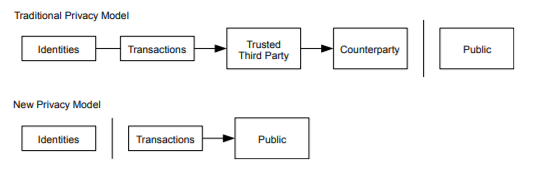
\includegraphics[width=1\textwidth]{Images/privacy}
	\caption{Blockchain privacy model \cite{Nakamoto_bitcoin}.}
	\label{privacy}
\end{figure}

Issues related to privacy may occur if identities are not properly secured, and transaction data is leaked to, or otherwise obtained by, unauthorized parties such as criminals or companies that exploit the data. E.g. criminals could monitor electricity consumption of a household to detect when the house is empty and thus rob it. With all the recent focus concerning data privacy, willingness to use such a system would diminish if transaction data was sold to companies that for instance used it to analyze user behavior and thereby using it for marketing and advertising.

One way to ensure that unauthorized people are not given access to data on the blockchain, could be to encrypt all the information that is stored on the blockchain, and only grant access to the decryption key to approved participants of the network. However, the encryption and decryption of data is a fairly heavy computationally operation, and leads to more overhead in the system. This also requires that all members of the network are given the decryption key. What would happen if someone accidentally (or purposely) gives away their key information? Such an implementation would require a careful and well tested design. 

%Asymmetric cryptography is also proposed as the method for signing the smart contracts. The need to protect private keys is also relevant in this case. 

%The implementation of smart contracts needs to be thoroughly verified before it is included in the system. Since smart contracts are stored on the blockchain, any weaknesses or faults of the contract is visible to anyone who has access to the blockchain. 

\section{Limitations in Implementation}\label{limit}
Blockchain technology is still very young, with the first appearance in 2008, in the Bitcoin white paper. The Ethereum platform, launched in 2015, is one of the very first to use the blockchain technology for something else than just crypto currency. In the past couple of years, there has been huge advantages in the field, and many new blockchain applications have been created. Furthermore, several of the papers used for the background research of this thesis have been published within the past year. 

Among the newer blockchain technologies is the Hyperledger platform. Version 1.0 was released in March 2017, and version 1.1 in March 2018. This platform has great potential for developing a system such as the one presented in this thesis. However, rather than spending a lot of time learning a specific framework, the goal was rather to learn the blockchain functionality, and this was done by implementing a blockchain form scratch. In retrospect, this might not have resulted in the best possible system. However, it has given tremendous insight in how blockchains work and their abilities, and more importantly - their limitations.

The advantages of building the blockchain structure from scratch is that it can be formed exactly how the system specifications require it to be. Furthermore, the system can be implemented without transaction fees, which would be required e.g. on the Ethereum platform. 

The disadvantages of not utilizing existing blockchain platforms is that it requires more extensive testing to ensure correct behavior, more maintenance, and more documentation. By using an existing blockchain platform, like Hyperledger Fabric, the development of the system would most likely be faster, seeing as the low-level modules are implemented, thoroughly tested, and ready for use. Hyperledger also has a built-in smart contract program in \textit{chaincode}. The modular architecture of Hyperledger Fabric presents the ability to design the system just as required.

 
\subsection*{Consensus}
As previously mentioned, the consensus module is not without flows, as became clear in the testing. Other issues regarding the module include the lack of protection against Byzantine nodes. It can be argued that in a consortium blockchain where nodes are validated, fault-tolerance is sufficient and the system does not need to be BFT. Furthermore, as such a system would be restricted to a limited physical area, it is quite likely that network participants are acquaintances in real life, thus reducing the risk of Byzantine nodes. Nonetheless, in the current implementation nodes are not part of the validation process, they simply require the IP address and port number of a node in the network. A brute force attack could quite easily access the network and establish itself as a leader by starting to send out \textit{append entries} messages.  

One of the big advantages of the RAFT protocol, apart from being very understandable and quite easy to implement, is that there are no possibilities for forks in the network, due to the strong consistency of the consensus protocol. Once a block is commited to the blockchain, it is commited by all nodes and no other block can be commited in its place. Another, and more important advantages, is that there is no need for any tokens or crypto currencies in the network. In contrast to the PoW protocol in the Bitcoin blockchain, which require enormous amounts energy to operate, the RAFT protocol is a lightweight protocol, that can run on normal processing capacity.

\subsection*{Network}
In the current implementation of the network module, all nodes have an open connection to all other nodes in the system. This solution does not scale well when the network is extended. One possibility to solve this problem could be to limit each node to e.g. 5 connections. This requires that all messages are broadcasted and forwarded until they have reached all nodes in the network and could be achieved by numbering all messages. 

On the other hand, the network protocol works very well. The \textit{Twisted} library eased the development of the network communication, as the low level components of the protocol were abstracted away. This allowed for a well structured and  modularized API. 
 
\subsection*{Smart Contracts}


\subsection*{Storage}
As shown in the results, a block containing energy transactions from 4 nodes resulted in approximately 423 bytes. With a new block created every minutes, this will eventually produce a large sized blockchain. A solution to this could be to limit the blockchain horizon to 3 years, which is how long power companies are required to store readings \cite{store}. Thus, after year 4, the first year worth of blocks will be removed from the blockchain and the genesis block rewritten to match the new first block of the blockchain. 


%Summary of what worked and what was not implemented due to time restrictions, what could have been done differently

\section{Future Work}\label{future}
%WHY IS THIS IMPORTANT?
Current implementation stores blockchain and other logs locally on machine, a future improvement could be to store the data in the cloud to save space.

To save space, blocks containing transactions that are settled or smart contracts that are no longer valid can be deleted. 

Make new users part of validation - to ensure true consortium. Current solution can be attacked through brute force, since the only requirement to join is to know the IP address and port number of an existing node on the network.

Automatic selection of who to initiate smart contract with for consumer based on pre-defined constraints 

Only some nodes part of validation? and let these have open connections to each other, let remaining nodes have connections to at least one of the validation nodes. 

Merkel trees for scalability. Is there a point though, since merkel trees are for time saving (?) and we are not iterating through blockchain to find previous transactions. Maybe usable in smart contract blockchain

Increase BFT by signing messages to prove authenticity.  -
Consensus: limit consensus nodes to only 5. 

Automatic smart contract based on pre-set prices given by prosumer and consumer

Settlement - better algorithm - including taking electricity from batteries for better flow

Hardware

Following is a summary of the future work that should be carried out on the system, based on what was discussed in this section and in section \ref{limit}.

\begin{itemize}
\item lolz
\end{itemize}